\documentclass[10pt,a4paper]{article}
\usepackage[T1]{fontenc}
\usepackage[utf8]{inputenc}
\usepackage{mathptmx}
\usepackage[left=2cm,right=2cm,top=1.8cm,bottom=1.8cm]{geometry}
\usepackage{amsmath,amssymb}
\usepackage{graphicx}
\usepackage{booktabs}
\usepackage{float}
\usepackage{array}
\usepackage{microtype}
\usepackage[font=small,labelfont=bf,skip=4pt]{caption}
\usepackage{titlesec}
\usepackage{enumitem}
\usepackage{xcolor}
\usepackage{listings}
\usepackage[hidelinks]{hyperref}

\titlespacing*{\section}{0pt}{6pt plus 2pt minus 1pt}{3pt}
\titlespacing*{\subsection}{0pt}{5pt plus 1pt minus 1pt}{2pt}
\titleformat{\section}{\normalfont\large\bfseries}{\thesection}{0.6em}{}
\titleformat{\subsection}{\normalfont\normalsize\bfseries}{\thesubsection}{0.6em}{}
\setlist[itemize]{topsep=2pt,itemsep=1pt,parsep=0pt,leftmargin=1.2em}
\setlist[enumerate]{topsep=2pt,itemsep=1pt,parsep=0pt,leftmargin=1.4em}
\setlength{\abovedisplayskip}{4pt}
\setlength{\belowdisplayskip}{4pt}
\setlength{\textfloatsep}{8pt}
\renewcommand{\arraystretch}{1.05}
\linespread{0.97}\selectfont

\lstset{basicstyle=\ttfamily\scriptsize, columns=fullflexible, keepspaces=true,
        breaklines=true, frame=lines, numbers=left, numberstyle=\tiny\color{gray},
        commentstyle=\color{gray}, stringstyle=\color{teal!70!black},
        keywordstyle=\bfseries, showstringspaces=false, upquote=true}

\title{\vspace{-1.2cm}\bfseries Biased Randomisation in a Savings-Based GRASP:\\
Four Selection Rules for the Travelling Salesman Problem}
\author{Heuristic Algorithms in Transport and Finance --- Master's course assignment \\
    Javier Salvatierra \\
    Jesús Inurria
}
\date{October 2026}

\begin{document}
\maketitle
\vspace{-0.8cm}

\begin{abstract}
\noindent\small
A GRASP repeats a randomised greedy construction and a local search. We build travelling salesman tours with the Clarke and Wright savings, improve
them with 2-opt and compare the classic uniform restricted candidate list (RCL) with four
\emph{biased randomisation} rules --- geometric, triangular, Zipf and softmax --- whose probability
decreases along the savings list. Each rule is tuned on three separate
instances and tested on seven TSPLIB instances with 51--280 cities, 20 runs of 150 iterations each.
GRASP lowers the mean gap of the greedy savings tour plus 2-opt from $5.07\,\%$ to
$2.22\,\%$; the geometric rule lowers it to $1.70\,\%$ at the same cost per run, and is significantly
better on two instances and never worse. A Friedman test across instances detects no global
difference ($p=0.76$).
\end{abstract}

\section{Introduction}

A salesman has to visit $n$ cities once each and return home along the shortest possible tour. This
is the Travelling Salesman Problem (TSP), the standard NP-hard routing problem: exact methods need specialised codes whose running time grows quickly
with $n$, so heuristics are used when a good tour is needed fast. A Greedy Randomized Adaptive Search Procedure (GRASP)~\cite{feo1995} is a multi-start method: every iteration builds a solution by choosing, at each step, one of the best candidates at random, improves it by local search, and the best solution is returned.

The classic GRASP draws uniformly from a \emph{restricted candidate list} (RCL). Juan et
al.~\cite{juan2011} used instead, in the savings heuristic of Clarke and Wright~\cite{cw1964}, a
geometric distribution over the positions of the sorted savings list, so that better candidates
are always more likely but none is excluded; this is \emph{biased randomisation}. We compare four biased rules with the classic RCL in a GRASP for the TSP, with everything else fixed. We deal only with the symmetric Euclidean TSP and a plain 2-opt local search.

The test instances are seven from TSPLIB~\cite{tsplib} whose optimal tours are published:
\texttt{eil51}, \texttt{berlin52}, \texttt{st70}, \texttt{eil76}, \texttt{kroA100}, \texttt{ch130}
and \texttt{a280}. The number in the name is the number of cities, so \texttt{a280} has $n=280$. All are of type \texttt{EUC\_2D} (city coordinates), and the optimum is the length of the companion tour \texttt{.opt.tour}. Below we state the model and the method, and report quality, time and significance tests.

\section{The TSP and the Clarke and Wright savings}
\label{sec:model}

Let $V=\{1,\dots,n\}$ be the cities and $d(i,j)=d(j,i)$ the Euclidean distance between $i$ and $j$,
rounded to the nearest integer as TSPLIB prescribes for its published optima. A tour is a permutation $\pi$ of $V$, and the TSP reads
\begin{equation}
\min_{\pi}\ \sum_{k=1}^{n} d(\pi_k,\pi_{k+1})
\qquad\text{s.t.}\qquad
\pi=(\pi_1,\dots,\pi_n)\ \text{is a permutation of } V,\qquad \pi_{n+1}=\pi_1 ,
\label{eq:model}
\end{equation}
i.e.\ every city is visited exactly once and the tour closes at its starting city.

Savings were designed for vehicle routing, with a depot. For the TSP we choose a
\emph{hub} $h$, the city closest to the centre of gravity of the coordinates, and start from the
\emph{dummy solution} that goes from $h$ to every other city and straight back. Serving two cities $i$ and
$j$ in sequence instead avoids one return to the hub and one departure from it, and saves
\begin{equation}
s(i,j) = d(h,i) + d(h,j) - d(i,j).
\label{eq:savings}
\end{equation}
By the triangle inequality $s(i,j)\ge0$ up to rounding; savings are largest for cities that are close
to each other and far from the hub. A saving depends only on $h$, $i$ and $j$, never on the partial
solution: as long as $i$ and $j$ are ends of different paths, both are still joined to the hub, and
linking them saves exactly $s(i,j)$. The $\binom{n-1}{2}$ savings are therefore computed and sorted in
decreasing order once per instance (4851 pairs for \texttt{kroA100}); this \emph{savings list} is the
candidate list of every GRASP iteration.

\section{GRASP with savings: RCL versus biased randomisation}
\label{sec:method}

The GRASP construction starts with every city except the hub as a path of its own and repeats three steps:
\begin{enumerate}
\item \textbf{Filter.} Keep only the pairs $(i,j)$ whose two cities are ends of their paths and lie on
different paths. Linking an interior city would create a branch; linking two ends of the same path
would close a cycle that skips the hub. A pair that fails can be deleted for good: paths only grow,
so an interior city stays interior and two cities on the same path stay together.
\item \textbf{Choose} a position $k$ in the filtered list (0 for the largest saving) with the
selection rule.
\item \textbf{Merge} the two paths through the chosen pair.
\end{enumerate}
After $n-2$ merges a single path covers the $n-1$ cities, and joining its two ends to the hub closes
the tour. The list shrinks after every merge, which is the \emph{adaptive} part of GRASP; always taking
the largest saving gives the classic savings heuristic. Let $m$ be the length of the filtered list and
$s_k$ its savings~\eqref{eq:savings}. The five rules are:
\begin{itemize}
\item \textbf{RCL (classic GRASP).} Uniform choice among the candidates with
$s_k\ge s_0-\alpha\,(s_0-s_{m-1})$: a hard cut-off on the \emph{value} of the saving.
\item \textbf{Geometric.} $P(k)\propto\beta(1-\beta)^k$, truncated to the $m$ positions; with
$\beta=0.4$ the best pair is chosen with probability $0.4$, the second with $0.24$.
\item \textbf{Triangular.} A density that decreases linearly over the first $L=\lceil f m\rceil$
positions (at least 3) and is zero afterwards.
\item \textbf{Zipf.} $P(k)\propto(k+1)^{-e}$, a power law with a heavier tail than the geometric one.
\item \textbf{Softmax.} $P(k)\propto\exp(z_k/T)$ with $z_k=(s_k-s_0)/(s_0-s_{m-1})\in[-1,0]$: it uses
the normalised \emph{value} of the saving, not its position.
\end{itemize}
The last four have no cut-off: every feasible pair keeps some probability. Geometric, triangular and Zipf look only at the rank, so their diversity does not
depend on how the saving values are distributed; the RCL and softmax do. Each rule has one parameter, between
greedy (every iteration builds the same tour) and nearly uniform (poor tours), that must be tuned.

The local search is \emph{2-opt}: for two non-adjacent edges $(a,b)$ and $(c,d)$ of the tour, if
$d(a,c)+d(b,d)<d(a,b)+d(c,d)$ the segment $b\dots c$ is reversed, so that $(a,c)$ and $(b,d)$ replace them. The first improving move is applied until none is left.

\section{Implementation}
\label{sec:impl}

The code is a single notebook, \texttt{GRASP\_TSP\_savings\_biased\_EN.ipynb}, in Python~3.13 with
NumPy, SciPy and pandas. The savings list is three arrays sorted with a stable sort. The construction keeps the degree and the path index of every city, so the filter of step~1 is one vectorised mask over the remaining list. The
geometric and triangular rules sample the position directly by inverting their distribution
functions; Zipf and softmax build a weight for every candidate and sample from the
cumulative sum. The 2-opt, sequential by nature, is compiled with \texttt{numba}.

\textbf{Tuning.} Every rule receives the same effort: a grid of 6--8 values from almost greedy to very
random, evaluated on three instances \emph{not} used for testing (\texttt{kroB100}, \texttt{eil101},
\texttt{ch150}; the optimum of \texttt{kroB100}, 22\,141, is fixed in the code) with 6 runs of 80 iterations and seeds different from the test ones. The value with the
lowest mean gap is kept: $\alpha=0.05$, $\beta=0.4$, $f=0.002$, $e=3$ and $T=0.02$, none at the edge of
its grid. Tuning took 306\,s. Juan et al.~\cite{juan2011} draw $\beta$ from $U(0.05,0.25)$ at every
selection, need no tuning and apply no local search; with 2-opt after every construction, our tuning
prefers a fixed and greedier $\beta=0.4$ (0.2 was also in the grid).

\textbf{Protocol.} Each rule runs 20 times on each test instance, 150 iterations per run, with seeds
$0,\dots,19$ shared by all rules, the same hub and the same 2-opt: 700 runs in 1011\,s. We record the
final cost (the objective of~\eqref{eq:model}), $\text{gap}=100\,(\text{cost}-\text{opt})/\text{opt}$, and the wall-clock time of the run
(150 constructions and local searches). Each biased rule is compared with the RCL instance by instance
with the two-sided Wilcoxon rank-sum test on the 20 final costs, with Holm correction over the 28
comparisons at the $5\,\%$ level; the Friedman test compares the five rules at once on the mean
gaps, with the instances as blocks. As a reference we also run the RCL with $\alpha=0$ (ties broken at random with a
fixed seed), with and without 2-opt, and check that each of these tours is a permutation of the
cities.

\section{Computational results}
\label{sec:res}

Table~\ref{tab:results} gives the mean gap of the 20 runs for every rule and instance, and Figure~\ref{fig:box} their distribution.

\begin{table}[!t]
\centering
\caption{Mean gap (\%) to the TSPLIB optimum over 20 runs of 150 iterations. \emph{CW}: greedy savings tour ($\alpha=0$),
without and with 2-opt. Superscripts: $^{+}$ significantly better, $^{-}$ significantly
worse than the RCL (Wilcoxon rank-sum, Holm, $5\,\%$). Last row: mean wall-clock time per run on
\texttt{a280}.}
\label{tab:results}
\scriptsize
\setlength{\tabcolsep}{5pt}
\begin{tabular}{@{}lrrrrrrrrr@{}}
\toprule
Instance & $n$ & Optimum & CW & CW + 2-opt & RCL & Geometric & Triangular & Zipf & Softmax \\
\midrule
\texttt{eil51}    & 51  & 426      & 5.40  & 4.46 & 1.41 & 1.10          & 0.95$^{+}$    & 1.20          & 1.41 \\
\texttt{berlin52} & 52  & 7\,542   & 11.06 & 6.58 & 3.69 & 0.93$^{+}$    & 2.04$^{+}$    & 3.35          & 3.44 \\
\texttt{st70}     & 70  & 675      & 4.74  & 3.56 & 0.82 & 1.01          & 0.99          & 1.26$^{-}$    & 0.93 \\
\texttt{eil76}    & 76  & 538      & 5.02  & 3.53 & 1.78 & 1.65          & 1.66          & 2.02          & 1.89 \\
\texttt{kroA100}  & 100 & 21\,282  & 6.04  & 3.18 & 0.94 & 1.14          & 1.12          & 1.19          & 0.91 \\
\texttt{ch130}    & 130 & 6\,110   & 7.28  & 4.70 & 1.71 & 1.73          & 1.80          & 1.54          & 1.46 \\
\texttt{a280}     & 280 & 2\,579   & 13.65 & 9.46 & 5.16 & 4.31$^{+}$    & 6.14$^{-}$    & 4.74          & 5.70 \\
\midrule
\textbf{Mean}     &     &          & \textbf{7.60} & \textbf{5.07} & \textbf{2.22} & \textbf{1.70} & \textbf{2.10} & \textbf{2.18} & \textbf{2.25} \\
Better/equal/worse vs.\ RCL & & & & & --- & 2/5/0 & 2/4/1 & 0/6/1 & 0/7/0 \\
Time per run, \texttt{a280} (s) & & & & & 5.81 & 5.33 & 5.53 & 10.18 & 9.93 \\
\bottomrule
\end{tabular}
\end{table}

\begin{figure}[!htb]
\centering
\graphicspath{{../results/figures/}}
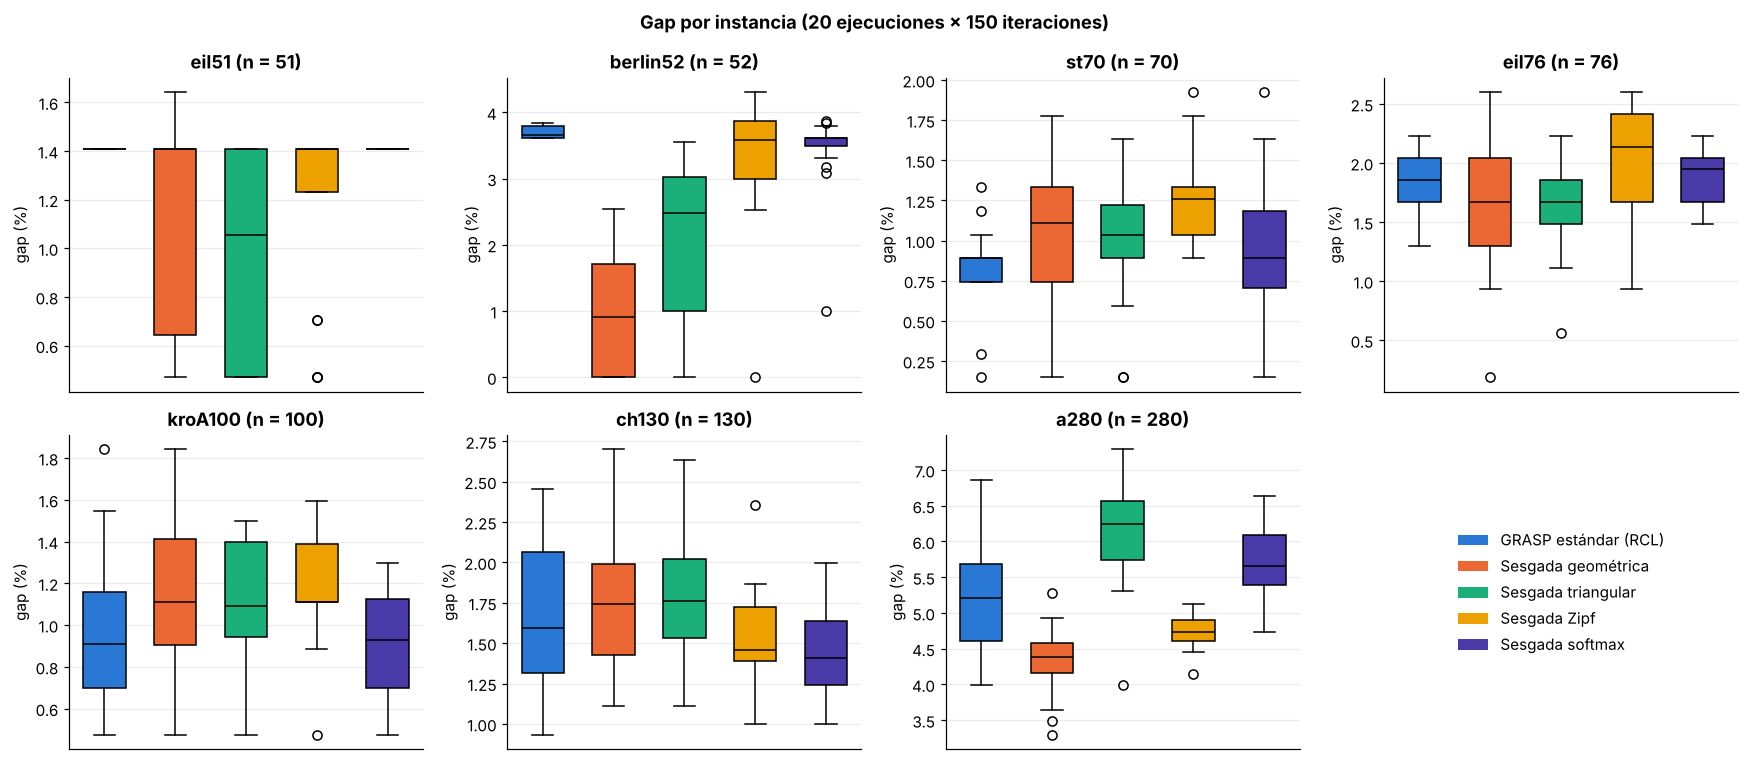
\includegraphics[width=0.85\textwidth]{gap_boxplots.png}
\caption{Gap (\%) of the 20 runs per instance and rule (boxes: quartiles and median; whiskers and
circles: spread and outliers). Colours, left to right: RCL (blue), geometric (orange), triangular
(green), Zipf (yellow) and softmax (purple). Panel and legend labels are in Spanish
(\emph{GRASP est\'andar} = RCL, \emph{Sesgada} = biased).}
\label{fig:box}
\end{figure}

\textbf{GRASP works.} The greedy savings tour ($\alpha=0$) is $7.60\,\%$ above the optimum on average, and
2-opt brings it to $5.07\,\%$. With a randomised construction and 150 iterations the mean gap falls to $2.10$--$2.25\,\%$ with any rule but the geometric one, and to $1.70\,\%$ with it; the classic GRASP alone removes $56\,\%$ of the error. The mechanism is
diversity: each randomised tour leads 2-opt to a different local optimum, and only the best of 150 is
kept.

\textbf{Geometric vs.\ RCL.} The geometric rule has the lowest mean gap, $23\,\%$ below the RCL, and
the lowest mean best gap over the 20 runs ($0.81\,\%$ against $1.70\,\%$ for the RCL). It is significantly better
on \texttt{berlin52} ($3.69\to0.93\,\%$) and \texttt{a280} ($5.16\to4.31\,\%$), equal on the other five
and never worse; a run of the geometric rule beats a run of the RCL (ties counted as one half) with mean
probability $0.60$. The reason is that the RCL cut-off is set on the normalised saving value, so the
number of candidates it admits depends on how the values are spread at the head of the list, and the
rule cannot be tuned per instance: on \texttt{eil51} the mean and the best gap of the RCL are both
$1.41\,\%$, so the 20 runs end in the same tour (the flat blue box in Figure~\ref{fig:box}), and on
\texttt{berlin52} the best of 20 runs is still $3.62\,\%$. A rank-based rule fixes the probability
of each position whatever the values are. 

\textbf{The other rules.} The triangular rule is mixed: better on \texttt{eil51} and \texttt{berlin52},
worse on \texttt{a280}, possibly because $f=0.002$, tuned on 100--150 cities, admits 78 positions at
the first step of \texttt{a280} against 10 on \texttt{kroB100}. Zipf is never better than the RCL and is worse on \texttt{st70}. Softmax is equal to the RCL on
all seven instances, and its \texttt{eil51} box is also flat. Both rules use the same normalised
value $z_k$, and with $T=0.02$ a candidate at $z_k=-0.05$, the edge of the RCL with $\alpha=0.05$,
weighs $e^{-2.5}\approx0.08$ relative to the best one: softmax is a smooth version of the same RCL.

\textbf{Time.} A run takes 0.14--10.18\,s, growing with $n$. The geometric and triangular rules cost the same as the RCL or less (0.77--0.95 times its time). Zipf and softmax, which weigh every feasible pair at every step, need 1.26--1.75 times the RCL time (about 10\,s against 5.81\,s on
\texttt{a280}). Times are means of 20 runs on one machine, comparable only with each other.

\textbf{Statistical caution.} The Friedman test over the seven instances gives $\chi^2=1.87$,
$p=0.76$: no global difference between the rules is detected. The evidence for the
geometric rule is moderate (two significant wins, none against), and the parameters were tuned on three instances with few runs.

\section{Conclusions}

With 2-opt, a GRASP built on the savings list more than halves the gap of the greedy savings tour ($5.07$ to $2.22\,\%$ with the classic RCL). Replacing the uniform
RCL by a geometric distribution over ranks lowers the mean gap to $1.70\,\%$ at no extra cost, because
its diversity does not depend on how the saving values are distributed; Zipf, softmax and the triangular rule do not
consistently improve on the RCL. The evidence is moderate: two significant wins and a non-significant Friedman test. The next steps are larger instances and more runs, a comparison at equal CPU
time, and a stronger local search, which may shrink the differences between rules.

\paragraph{Code availability.} All computations are reproducible from the notebook
\texttt{GRASP\_TSP\_savings\_biased\_EN.ipynb}, delivered separately (tuning about 5\,min, experiment
about 17\,min on our machine).

\begin{thebibliography}{9}
\footnotesize\setlength{\itemsep}{0pt}\setlength{\parskip}{0pt}
\bibitem{cw1964} G.~Clarke and J.~W. Wright. Scheduling of vehicles from a central depot to a number of
delivery points. \emph{Oper.\ Res.}, 12(4):568--581, 1964.
\bibitem{feo1995} T.~A. Feo and M.~G.~C. Resende. Greedy randomized adaptive search procedures.
\emph{J.\ Global Optim.}, 6:109--133, 1995.
\bibitem{juan2011} A.~A. Juan, J.~Faulín, J.~Jorba, D.~Riera, D.~Masip and B.~Barrios. On the use of Monte
Carlo simulation, cache and splitting techniques to improve the Clarke and Wright savings heuristics.
\emph{J.\ Oper.\ Res.\ Soc.}, 62(6):1085--1097, 2011.
\bibitem{tsplib} G.~Reinelt. TSPLIB --- a traveling salesman problem library. \emph{ORSA J.\ Comput.},
3(4):376--384, 1991.
\end{thebibliography}

\end{document}
